\chapter{Introduction}\label{C:intro}

\section{Problem Statement}
\emph{Service-oriented computing} (SOC) is a novel computing paradigm that employs services as fundamental elements to achieve the agile development of cost-efficient and integrable enterprise applications in heterogeneous environments \cite{papazoglou2003service, papazoglou2006p}. One of the primary purposes of SOC is to overcome conflicts due to diverse platforms and programming languages to make integrable and seamless communication among those existing or newly built independent services. \emph{Service Oriented Architecture} (SOA)  could abstractly realise service-oriented paradigm of computing. This accomplishment has been contributing to reuse of software components, from the concept of functions to units and from units to services during the evolution of development in SOA \cite{booth2004web, overdick2007resource}. One of the most typical implementation of SOA is \emph{web service}, which designated as ``modular, self-describing, self-contained applications that are available on the Internet" \cite{curbera2001web}. Several standards play a significant role in registering, enquiring and grounding web services across the web, such as UDDI \cite{curbera2002unraveling}, WSDL \cite{lausen2007semantic} and SOAP \cite{fensel2011semantic}. \emph{Web service composition} aims to loosely couple a set of web services to provide a value-added composite service that accommodates complex functional and non-functional requirements of service users. 

Two most notable challenges for web service composition are ensuring interoperability of services and achieving Quality of Service (QoS) optimisation \cite{fensel2011semantic}. \emph{Interoperability} of web services presents challenge in syntactic and semantic dimensions. The syntactic dimension is covered by the XML-based technologies \cite{yu2008deploying}, such as the previously discussed $WSDL$ and $SOAP$. In this dimension, most of service compositions are merely based on the matching of input-output parameters. The semantic dimension enables a better collaboration through ontology-based semantics \cite{o2005review}, in which many standards have been established in this dimension. E.g., OWL-S \cite{martin2004owl}, Web Service Modeling Ontology (WSMO) \cite{lausen2005w3c}, SAWSDL \cite{kopecky2007sawsdl}, Semantic Web Services Ontology (SWSO) \cite{petrie2016web}. This dimension bring around some other services' resources that could effect the execution of web services and their composition (i.e., precondition and postcondition). On the whole, these two challenges give birth to \emph{Semantic web services composition} and \emph{QoS-aware service composition}. \emph{Semantic web services composition} is distinguished from the tranditional service composition (i.e., only syntactic dimension presented in web services). The resources of semantic web services are described semantically to enable a better interoperability for chaining web services. Another challenge is related to QoS optimisation. E.g., minimum cost and maximum reliability. This problem gives birth to \emph{QoS-aware service composition} that aims to find composition solutions with optimised QoS. 

Further more, the environment of service composition is changing in the real world, rather than \emph{static}. E.g, QoS values of services being composed of are fluctuating over time, or service chosen at the planning stage may not avaible to be invoked at the runtime. Most of importance is \emph{static web service composition} supports the environment change badlly because of outdated composition solutions. Therefore, \emph{Dynamic web service composition} become a very demanding research field with a growing interest for providing solutions that adapt to the changing environment. Additionly, in context of semantic web service composition, semantics of web services can make the problem of dynamic web service composition more complicated for the changing ontology.


Different approaches have been proposed to solve those composition problems discussed above and they can be classified into two main categories: \emph{semi-automated web service composition} and \emph{fully automated web service composition}. The first composition problem requires human beings to manually create abstract workflows. Generally, researchers assume the pre-defined abstract workflow is given and provided by the users. The optimisation problem in this approach turns to selecting the concrete services with the best possible quality to each slot of the given workflow. Due to a tremendous growth in industries and enterprise applications, the number of web services has increased dramatically and unprecedentedly. The process of conducting abstract workflows  manually is fraught with difficulties. Therefore, fully automation of the composition process was introduced in web service composition for less human intervention, less time consumption, and high productivity. The advantages of fully automated approach is that an abstract workflow is not not provided, but it is established while service are selected. 


Generating composition plans automatically in discovering and selecting suitable web services is a NP-hard problem \cite{moghaddam2014service}, which means the composition solution is not likely to be found with reasonable computation times in a large searching space. \emph{Artificial Intelligence (AI) planning-based approaches}, \emph{Evolutionary Computation (EC) techniques} and hybrid techniques  are introduced to handle this problem. AI planning problem is solved in making a plan, from initial states to a set of actions to desired goal states-composite web services, where services are considered as actions triggered by one state (i.e., inputs) and resulted in another state (i.e., outputs). In the second approach, heuristics have to be employed to generate near-optimal solutions, where a variety of EC techniques have been used in this context. E.g., Genetic Algorithms (GA), Genetic Programming (GP) and Particle Swarm Optimisation (PSO). EC-based techniques have been effectively proposed to solve \emph{QoS-aware web service composition} problems with different designed data structures for representation. Recently, different solution representation utilised in different EC-based method have been investigated in QoS-aware web service composition problems, since they could significantly impact on the performance while performing fully automated service composition. In the third approach, a hybrid of AI planning-based approaches and EC-based approaches are proposed to fulfil the correctness in constructing workflows with users' constraints, while the quality of composition solutions are also optimised according to users' requirement.

The overall goal of this thesis is to propose a comprehensive-quality aware automated web service composition. This comprehensive quality aims to jointly optimise semantic matchmaking quality and QoS. Meanwhile, this new approach also tackles serveral service composition problems, such as semantic web service compostion, multi-objective optimisation, dynamic web service composition.

\section{Motivations}
The motivations of automated semantic web service composition lies in the requirements from three key aspects that simultaneously account for. 
\begin{enumerate*}
 \item \emph{Quality of service composition}: previous studies have suggested many approaches to optimise QoS, which refers to the non-functional quality of service composition. However, the importance of the functional quality (i.e, semantic matchmaking quality) are not recognised in these works.
 \item \emph{Composition constructs}:
 \item \emph{dynamic service composition}:
\end{enumerate*}
Herein these requirements are explicitly discussed below. 

\subsubsection{Hybridisation of Quality of Semantic Matchmaking and Quality of Service}
Often, many different service compositions can meet a user request but differ significantly in terms of QoS and semantic matchmaking quality. For example, in the classical travel planning context, some component service must be employed to obtain a travel map. Suppose that two services can be considered for this purpose. One service $S$ can provide a street map at a price of 6.72. The other service $S'$ can provide a tourist map at a price of 16.87. Because in our context a tourist map is more desirable than a street map, $S'$ clearly enjoys better semantic matchmaking quality than $S$ but will have negative impact on the QoS of the service composition (i.e., the price is much higher). One can easily imagine that similar challenges frequently occur when looking for service compositions. Hence, a good balance between QoS and semantic matchmaking quality is called for.

Existing works on service composition focus mainly on addressing only one quality aspect discussed above. For the semantic matchmaking quality, it is mainly addressed in the discovery of an atomic service. I.e., one-to-one matching of user requirements to a single service. The service composition \cite{bansal2016generalized,boustil2014semantic,mier2015integrated} utilised semantic descriptions of web services (e.g., description logic) to ensure the interoperability of web services, but the goal of the composition is often to minimise the number of services or the size of a graph representation for a web service composition. These approaches do not guarantee an optimised QoS of service compositions. On the other hand, huge efforts have been devoted to studying QoS-aware web service composition, and some approaches to QoS-aware web service composition do consider the semantic matchmaking while composing solutions, but they do not recognise the importance of semantic matchmaking quality. For these reasons, there is a need to device an automated approach for jointly optimising the two quality aspects.


\subsubsection{Multi-Objective Composition Optimisation}
Web service compostion problems fall into two groups, depending on an optimisation for a single objective or multiple objectives. In single-objective service compositions, a single composition solution is always returned by the composition task, when the preferences of each quality conponent within the single objective (e.g., a weighted sum of different quality criteria) is known by users. However, users do not always have clear preferences when many quality criteria are presented. Therefore, multi-objective is a natural features of requirements from users to provide a set of trade-off solutions for the conflicting quality criteria. E.g., Premium users do not care cost as much as price-sensitive users do, so they may prefer a composition solution with lowest execution time,  rather than one with a relatively lower execution time without exceeding a budget. Therefore, a multi-objective  fully automated service composition approach is very demanding.

Existing research on the automated web service compostion mainly contrates on sigle objective problems for QoS-aware web service compositions. I.e., there is only one solution promoted by a unified QoS ranking score to all the users. However, in multi-objective context, service composition problems  \cite{liu2005dynamic,wada2012e3,yin2014hybrid} are only approached by semi-automated methods, where the workflow structure is assumed to be pre-existing. These approaches handle the conflicting QoS attributes independently. From above discussion, these is a lack of fully automated approaches to multi-objective web service composition problems. Moreover, the insufficiency of handling only non-functional attributes (i.e., QoS) has given rise to adding semantic matchmaking quality into consideration.

\subsubsection{Automated Web Service Composition Based on Preconditions and Effects}
Apart from considering the satisfactory inputs and production of outputs, some conditional constraints also determine the execution of services.  These conditional constraints lead to multiple possible paths for execution when services are composed together. E.g., In the scenario of an online book shopping system adapted from \cite{wang2014automated}, services are composed to provide an operation for book shopping.  Users expect that purchase outcome (e.g. receipt) is returned If book and customer details (e.g. title, author, customer id) are given. In this case, the users may have specific constraints. if the customer has enough money to pay for the book in full, then they would like to do so. Otherwise, the customer would like to pay by instalments. The constraints are on their current account balance.






Most approaches for automated web service composition represent web servicess through inputs and ouputs. The matching of inputs and outputs of services is simpliy utilised to achieve service composition. However, inputs and outputs only specify the data/information transformation of services \cite{martin2004owl}, while the underlying functional knowledge of services are not included \cite{paliwal2012semantics}. Therefore, besides inputs and outputs, web services in the real world may need some prerequisties for execution, and result in some changes. Especially, the resulting changes of services may be nondeterministic. All these requirements for service execution are should not be ignored, as they impact the actual execution of web services and the service composition. Despite many promising approaches for automated web service composition, the prerequisties and resulting changes (often know as precondition and effects) are not well studied and fully used in the prior approaches. 






%The intricacy of Web service composition lies in the number of distinct facets it must simultaneously account for. As the \textbf{first facet}, services must be combined so that their operation inputs and outputs are properly linked, i.e. the output produced by a given service is usable as input by the next services in the composition, eventually leading up to the desired overall output. As the \textbf{second facet}, services must be arranged appropriately in the composition according to the desired outcome (e.g. in sequence, in parallel). Particular attention must be paid to conditional constraints, when the composition is required to have multiple execution options -- branches -- according to a given condition \cite{wang2014automated,sohrabi2009web,karakoc2009composing}. As the \textbf{third facet}, the composition must achieve the best possible overall Quality of Service (QoS) with regards to attributes such as the time required to execute the composite services, the financial cost of utilising the service modules, and the reliability of those modules. As the \textbf{fourth facet}, the environment of the composition must be recognised as dynamic, with QoS values that fluctuate and services that become unavailable/available over time. These facets are discussed in more detail below:

\begin{enumerate}


 %\item \textbf{Service attributes:} Functional solutions are compositions where connected services are well-matched, that is, the inputs of each service are completely satisfied by the outputs of other services, executed earlier in the workflow. In order to ensure functionality, two main approaches can be used: \emph{immediate} and \emph{gradual}. Whenever a solution is built using immediate approaches, this solution is fully functional, i.e. the inputs of all atomic services are fully satisfied, and so are the overall task outputs given the provided inputs. This is typically done by employing AI planning algorithms that verify the correctness and completeness of the connections between services at every building step \cite{wang2014automated}. When a solution is built using gradual approaches, on the other hand, there are no guarantees that it will be fully functional. As opposed to performing checks at every building step, gradual approaches rely on the notion of improving solutions over multiple iterations, each time penalising incorrect and/or incomplete connections between services. In practice, these approaches are typically implemented using Evolutionary Computation techniques with penalties enforced through the fitness function \cite{rodriguez2010composition}. The simplest way of establishing that the inputs of an atomic service have been satisfied is by verifying that there is an exact type match between each target input and its corresponding incoming connection (i.e. the output of a previous service). However, a more sophisticated matching approach relies on measuring the semantic similarity between the output and input types in question with the help of an ontology \cite{DBLP:journals/soca/BoustilMS14}; in this case, the smaller the distance between the two values, the better the match.
 %\textbf{Quality of Service:} Quality of Service (QoS) refers to the non-functional (quality) attributes associated with a Web service, such as its expected execution time when answering requests, its availability, and its scalability \cite{ko2008quality}. The overall quality of compositions can be measured by aggregating the individual QoS values of its constituting atomic services, meaning that it is possible to optimise the composition's QoS by selecting the right combination of constituting services. As mentioned earlier, the selection of a set of services in order to maximise the overall QoS can be mapped into a classic optimisation scenario, and this has been done extensively in the literature. A variety of EC techniques have been used in this context \cite{wang2012survey}, as well as other optimisation techniques such as integer linear programming \cite{yoo2008web}. Interestingly, AI planning techniques were also used to this end, even though in this case they are incapable of also considering conditional constraints \cite{deng2013efficient}. In the realm of QoS optimisation, multi-objective techniques are often employed to the problem of Web service composition, since the optimisation of potentially conflicting QoS attributes such as time and cost is more intuitively performed using independent objective functions \cite{liu2005dynamic}. An extension to the problem of QoS-aware composition is that of SLA-aware Web service composition \cite{yin2014hybrid}, where solutions must not only be quality-optimised but also abide by minimum quality standards (i.e. thresholds) defined by the composition requestor. SLA-aware composition has focused on tasks with a single execution path, but research still must be conducted on those with multiple execution paths (i.e. tasks with conditional constraints).

 
 %\item \textbf{Composition constructs:} In addition to considering the functionality of services within the composition, it is necessary to arrange them appropriately. This ensures, for example, that services that depend on each other are sequentially connected, while services that are independent from each other are allowed to be executed in parallel. Another fundamental construct is a conditional constraint, which determines when the execution of a composition should branch into one of multiple possible paths, depending on runtime values. For example, consider the scenario of an online book shopping system, adapted from \cite{wang2014automated}. In this scenario, the objective is to employ existing Web services to accomplish a basic book shopping operation. Preferably, the services to be used, the order in which they are to be invoked, and how they interact with each other should be determined automatically. Therefore, the book and customer details (e.g. title, author, customer information) and the expected purchase outcome (e.g. receipt) act as the composition task inputs and outputs, and the shopping-related services as the atomic composition components. In certain cases, however, the customer may have specific constraints. For example, the customer's preferred method of payment is likely to depend on their current account balance: if the customer has enough money to pay for the book in full, then they would like to do so, otherwise the customer would like to pay by installments. In this case, the composition task has one set of inputs (book and customer details), and a condition (balance) that may lead to two different sets of outputs depending on whether it is met (either a receipt for paying in full or the initial installment bill). In this type of composition, the runtime value of the type in the condition is used to ultimately decide which set of outputs should be produced. Different techniques have been explored to achieve compositions that consider conditional constraints, including the use of AI planning with rules encoding user constraints \cite{DBLP:journals/soca/BoustilMS14} and the representation of the composition as a constraint satisfaction problem to be processed with a solver engine \cite{karakoc2009composing}. This territory has not been widely explored by applying Evolutionary Computation (EC) techniques; yet, due to their flexibility and efficiency, it would be interesting to focus on the investigation of ways in which to extend them to apply these constraints.
 
 
 \item \textbf{Dynamic composition:} In a more realistic scenario, Web service compositions exist within a dynamic environment where the quality and availability of the atomic services in the repository varies as time passes. In such a dynamic environment, providing a static composition solution to a task is no longer enough, since this solution may decrease in quality throughout time and/or become non-executable if some of its composing services go offline. Thus, the focus of dynamic Web service composition is on monitoring and updating composition solutions as they become outdated \cite{li2014fault}. The majority of techniques aimed at updating outdated or faulty compositions rely on building solutions that present constructs allowing for dynamic adaptation \cite{alferez2014dynamic}, but not many EC-based approaches have been tried in this area.
\end{enumerate}

The above discussion refers to several techniques that have been proposed to address the composition problem \cite{rao2005survey}. These techniques produce promising results,
however they do not account foll all of these composition facets at once. For example, AI planning techniques for composition \cite{huang2009effective,deng2013efficient} focus on guaranteeing functional correctness (first facet), and either fulfilling conditional constraints (second facet) or optimising QoS (third facet); similarly, EC techniques such as Genetic Algorithms (GA) and Genetic Programming (GP) \cite{rodriguez2010composition,wang2012survey} focus on QoS in addition to functional correctness, but do not include the fulfilment of conditional constraints.

\subsection{Limitations of Current Web Service Composition Approaches}


Traditionally, AI planning and EC have been employed separately to solve the problem of Web service composition. On the one hand, AI planning techniques are outstanding at ensuring the creation of composition solutions that have appropriate connections between the outputs and inputs of the composing services, and also at ensuring the creation of branches according to the constraints provided. On the other hand, EC techniques are ideal for encountering solutions with a good overall quality amongst a very large array of possibilities. Given the strengths of each set of techniques, it would be advantageous to combine these two composition strategies into a single approach that offers both sets of capabilities, and thus considers more service composition facets simultaneously. In this hybrid approach, users would be able to specify the conditions of when branching should occur, the order in which these conditions should be observed, and the outputs each execution branch should produce; the technique would then return a suitable solution. Despite being a promising approach, this area has currently not been investigated in depth.

\subsubsection{Multi-Objective Composition Optimisation}

\subsubsection{Semantic Web Service Selection}
When building a candidate composition solution, atomic services must be selected according to the compatibility of their inputs. The simplest form of selection is when the inputs of services are matched according to their exact type, though recently more sophisticated semantic approaches that also allow for inexact matches have been investigated. In a typical selection scenario, a concrete service is chosen to fulfil the functionality specified by an already-defined abstract service, which restricts the complexity of the problem. However, the concept of an abstract service cannot be used when selecting services during an AI planning-based composition, which decreases the efficiency of this approach. As this problem has not been addressed in current works, a better way of performing semantic selection must be proposed for use with AI planning-based composition approaches.

\subsubsection{EC-based Dynamic Web Service Composition}
Evolutionary Computation (EC) approaches to Web service composition have been extensively investigated in static scenarios, where the quality and availability of services are assumed to remain constant, however the use of these techniques has only been superficially explored in dynamic scenarios. Despite this lack of research, EC-based approaches show promise in the area of dynamic Web service composition for two reasons: firstly, they allow a composite service system to \emph{self-heal} by maintaining a population of solutions and using them as alternative compositions in the case of failure; secondly, they support \emph{dynamic adaptation} by allowing solutions to be further evolved in order to account for changes in the QoS values of atomic services. Given these advantages, it is desirable to investigate the use of EC approaches in a dynamic composition context.

\section{Research Goals}
The overall goal of this thesis is to propose a hybrid  Web service composition approach that considers elements from all four facets described above when generating solutions. More specifically, this approach combines elements of AI planning, to ensure functional correctness and constraint fulfilment, and of Evolutionary Computation, to evolve a population of near-optimised solutions from a QoS standpoint. The research aims to determine a flexible way in which planning and EC can be combined to allow the creation of solutions to solve composition problems that require multiple execution paths. The research goal described above can be achieved by completing the following set of objectives, outlined in Figure \ref{fig:objectives}, which are intended to be used as research guides throughout this project:

 \begin{figure}
\centerline{
\fbox{
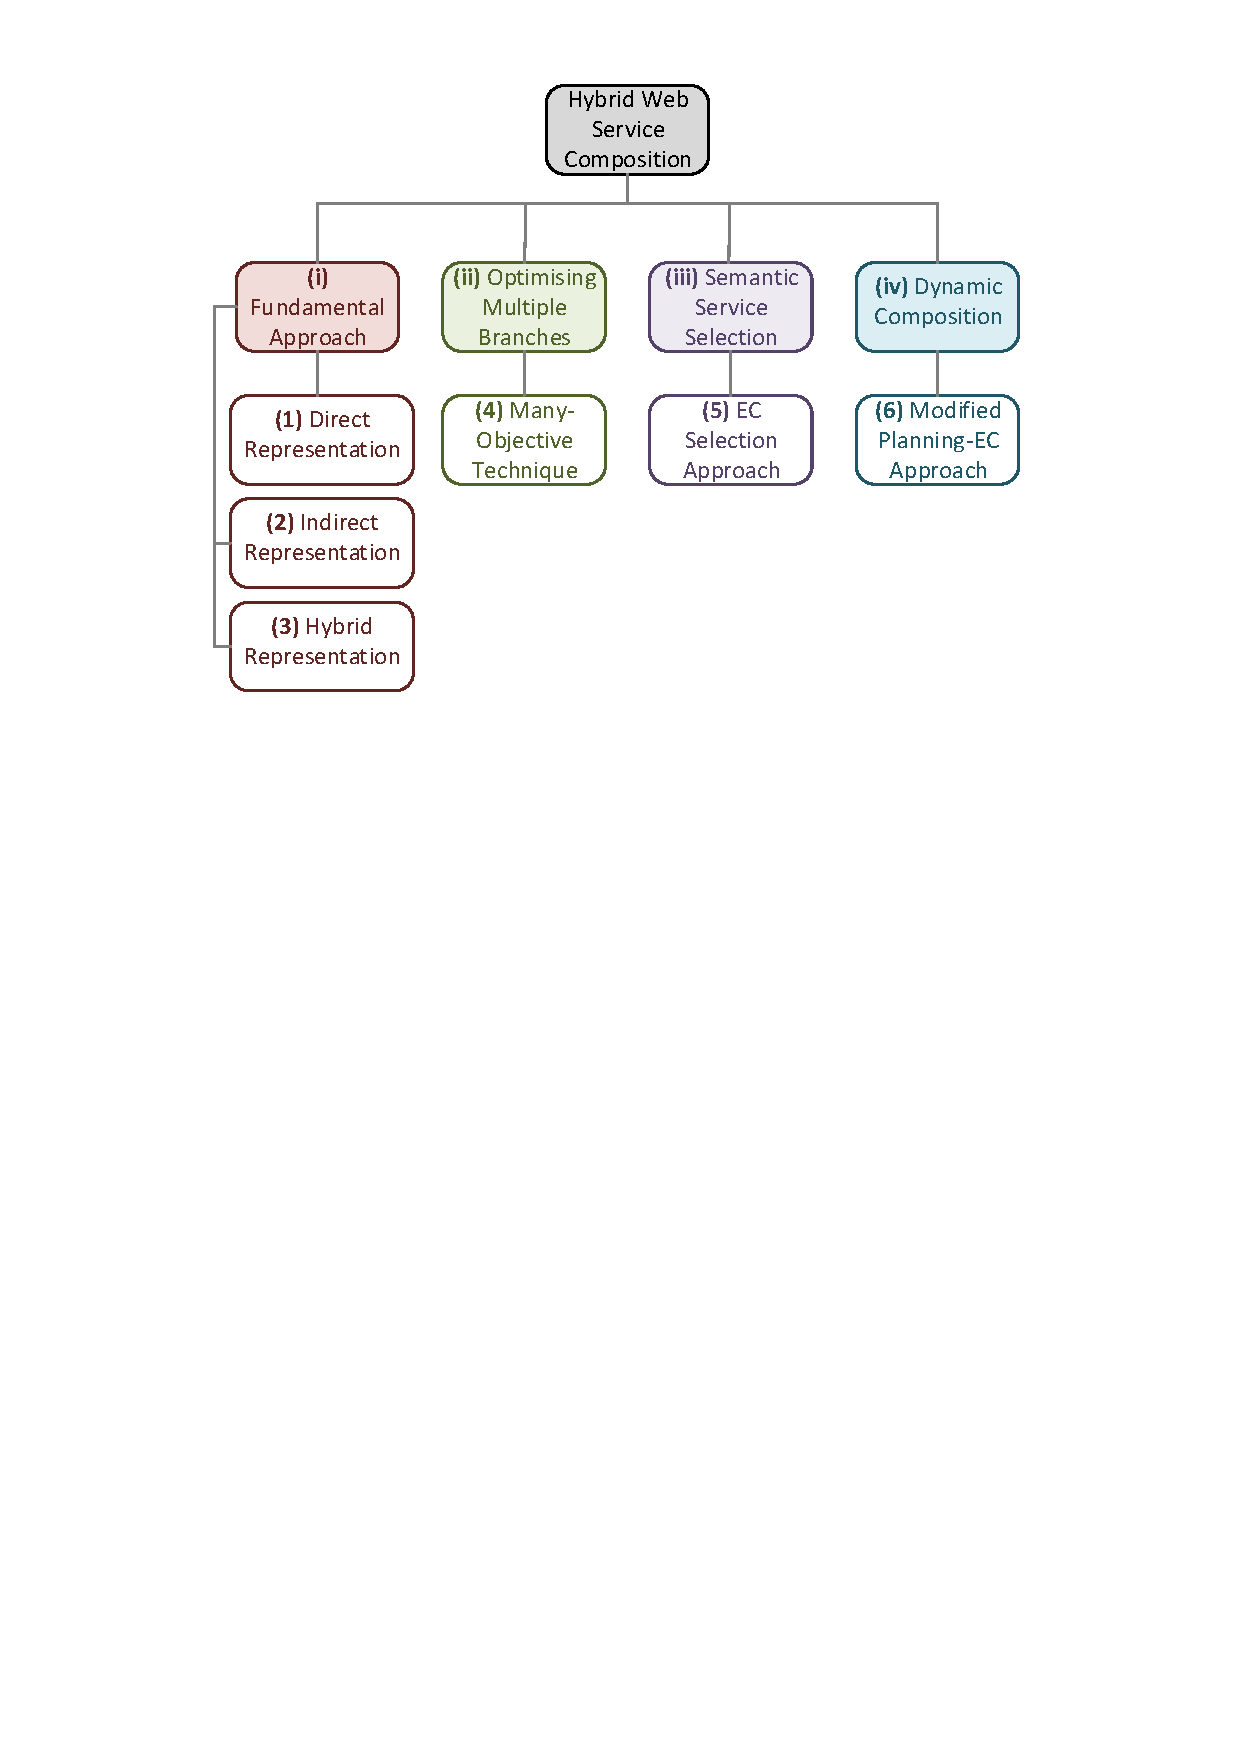
\includegraphics[width=12cm]{objectives.pdf}
}}
\caption{Research objectives and sub-objectives.}
\label{fig:objectives}
\end{figure}

\begin{enumerate}
   \item multiple constructs 
 \item multiple constructs. quality for precondition and effects
  \item \label{obj:rep} Create a hybrid QoS-aware Web service composition technique that combines elements of AI planning and evolutionary computation to allow for the optimisation of composition solutions with conditional constraints. One of the key aspects of this technique is the representation of each composition solution. Undoubtedly the simplest model would be that of a linear vector, with each element being a service that should be included into the composition, however this linear structure does not satisfactorily encode the relationships and links between different services. Another problem with a vector is that the EC techniques which use such a representation do not allow for structures of varying lengths, a requirement when performing fully automated composition. The search for a suitable solution representation leads to the following three sub-objectives:
  
  \begin{enumerate}
    \item \label{obj:direct} \emph{Propose a direct solution representation for the planning and EC-based Web service composition technique.}\\
    A tree or graph representation is well-suited to represent Web service composition solutions with conditional constraints, since such structures are naturally capable of representing the links between the composing services and multiple execution paths. These structures may be referred to as \emph{direct representations} of solutions, since the genotype and the phenotype of each solution are the same, meaning that solutions are represented directly as they should be interpreted. Proposing a representation based on these structures involves some trade-offs that must be carefully considered, such as the existence of EC techniques that support that structure and the computational cost they incur.
    \item \label{obj:indirect} \emph{Propose an indirect solution representation for the planning and EC-based Web service composition technique.}\\
    Despite the intuitiveness of direct representations, it has been argued in the problem domain of scheduling that indirect representations, where the final result must be decoded from a population candidate, have been shown to have better search performance than their direct counterparts \cite{hart2005evolutionary,craenen2001handle}. Due to this evidence, an indirect candidate representation should be proposed and compared to the direct representation. This indirect representation could be based on the Web service composition Particle Swarm Optimisation (PSO) approach proposed in \cite{da2014graph}.
    \item \label{obj:hybrid} \emph{Propose a hybrid solution representation for the planning and EC-based Web service composition technique.}\\
    In case there is a trade-off between the execution time and the quality of the solutions produced by the direct and indirect representations developed in Objectives \ref{obj:direct} and \ref{obj:indirect}, a hybrid representation should be proposed to combine the strengths of these two approaches. This representation could comprise the structure used in the direct representation with the addition of weights from the indirect representation. Comparisons should be performed to determine whether the hybrid solution presents any performance or quality gains.
  \end{enumerate}
 
 \item \label{obj:mo} Develop a many-objective (MO) approach to optimising the quality of candidate compositions with multiple execution paths, abiding by SLA constraints. Two factors must be taken into account when optimising Web service compositions with multiple execution paths: firstly, each Quality of Service (QoS) attribute must be optimised independently, since they may be conflicting with each other; secondly, each path of the composition must also be independently considered, since the QoS values for each path may vary significantly. The development of this approach can be divided into the following two sub-objectives:
 
   \begin{enumerate}
    \item \label{obj:simple-mo} \emph{Propose an unconstrained MO approach for independently optimising the execution paths of a Web service composition solution with conditional constraints.}\\
    The challenge in optimising compositions with multiple execution paths, while at the same time considering several independent quality measures, is the number of dimensions that must be considered simultaneously. On the one hand, encoding each individual quality measure of each execution path as an independent value provides the a very expressive representation of the problem; on the other hand, MO optimisation with a large number of dimensions may result in a solution set that contains many unremarkable solutions. Thus, the proposed approach must handle this issue.
    \item \label{obj:sla-mo} \emph{Extend this MO approach to also consider SLA constraints.}\\
    Once the fundamental MO optimisation approach has been proposed, it should be extended to observe SLA constraints. Note that these constraints must be enforced for each execution path individually, to ensure that all runtime options have been optimised according to the quality parameters of the composition requestor.
   \end{enumerate}
 
 \item \label{obj:semantic} Develop an EC technique for performing semantic Web service selection in the context of a planning-based composition technique. As discussed in Objective \ref{obj:rep}, the composition technique investigated in this thesis combines elements of AI planning and of EC approaches to achieve compositions that are correct, have conditional constraints, and can be optimised according to their QoS attributes. In planning-based approaches to service composition, however, the semantic selection process of candidate atomic services is inefficient, since there are many possible service matches to consider at each planning step. In fact, it may be unfeasible to consider all possible service matches in an exhaustive manner when handling larger service repositories, which invites the use of non-exhaustive approaches such as EC techniques to accomplish this task. Thus, this objective entails the use of an optimisation technique to discover semantically matching services to be included in a composition candidate. Note that this objective aims to investigate the use of an optimisation technique nested within the service selection step of the planning/EC approach.
 
 \item \label{obj:dyna} Modify the planning/EC composition technique to work in a dynamic environment. In a static scenario the planning-EC technique is executed once for a given composition task, returning a composite result under the assumption that the quality levels and the availability of the atomic services included in that result will remain constant. In a more realistic dynamic scenario, however, the quality of the services in the repository may fluctuate and occasionally services may become unavailable. To account for these setbacks, solutions must be corrected and updated in response to changes in the environment. In order to do this, the planning-EC technique is to be modified to retain a population of candidates as alternatives in case of failure, and further generations are to be evolved as the QoS values of services in the repository change, thus leveraging the natural features of Evolutionary Computation. These improvements are to be performed in two steps:
 
 \begin{enumerate}
 \item \label{obj:dyna-qos} \emph{Extend planning/EC technique to re-optimise candidates as the quality values of services changes.}\\
 Usually, EC approaches dedicated to Web service composition create a population of candidates, optimise this population, and identify the best solution candidate, discarding the others in the process. In a dynamic scenario, disposing of the remaining candidates would be wasteful, since some of these alternative solutions may become promising as quality values change. Instead of destroying the population, the extended technique should maintain it for future re-optimisation. A key challenge in this approach is striking a balance between population diversity and effective optimisation.
 \item \label{obj:dyna-fail} \emph{Create a strategy for handling service failure using other candidates in the population.}\\
 In addition to quality changes, the atomic services used in a composition may occasionally fail/become unavailable. An alternative execution plan must be used to prevent the composite service from being impacted, and the proposed solution is to select as efficiently as possible an unaffected candidate from the population as the replacement.
 \end{enumerate}
 
\end{enumerate}

%\section{Published Papers}

%During the initial stage of this research, some investigation was carried out on the suitability of different candidate representations for EC-based Web service composition. This culminated in the publication of the following papers:

%\begin{itemize}
% \item Alexandre Sawczuk Da Silva, Hui Ma and Mengjie Zhang. "A GP Approach to QoS-Aware Web Service Composition and Selection". \emph{Proceedings of the 10th International Conference on Simulated Evolution and Learning (SEAL 2014). Lecture Notes in Computer Science}. Vol. 8886. Dunedin, New Zealand. December 15-18, 2014. pp. 180-191.
% \item Alexandre Sawczuk da Silva, Hui Ma and Mengjie Zhang. "A GP Approach to QoS-Aware Web Service Composition including Conditional Constraints". \emph{Proceedings of 2015 IEEE Congress on Evolutionary Computation (CEC 2015)}. Sendai, Japan. 25-28 May, 2015 (To Appear)
% \item Alexandre Sawczuk da Silva, Hui Ma and Mengjie Zhang. "GraphEvol: A Graph Evolution Technique for Web Service Composition". \emph{Proceedings of the 26th International Conference on Database and Expert System Applications (DEXA 2015)}. Valencia, Spain. 1-4 September, 2015 (Accepted)
%\end{itemize}


\section{Organisation of Proposal}
The remainder of the proposal is organised as follows: Chapter \ref{C:review} provides a fundamental definition of the Web service composition problem and performs a literature review covering a range of works in this field; Chapter \ref{C:preliminary} discusses the preliminary work carried out to explore the hybridisation of AI planning techniques and EC-based techniques for Web service composition, one of the key ideas proposed in this project; Chapter \ref{C:plan} presents a plan detailing this project's intended contributions, a project timeline, and a thesis outline.
